\section{Przegląd istniejących symulatorów robota Velma} 

\begin{frame}
    \frametitle{Część manipulacyjna Velbody}
    \begin{figure}
        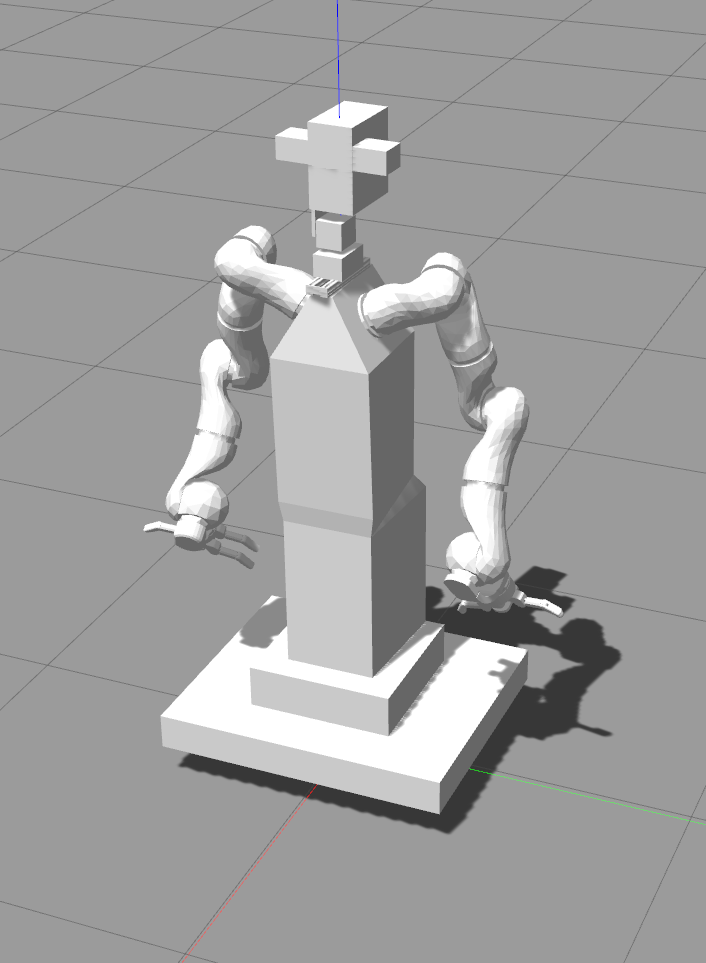
\includegraphics[scale=0.20]{./images/velma_gz_cropped.png}
        \caption{\normalsize{Część manipulacyjna robota Velma w symulatorze Gazebo}}
    \end{figure}
\end{frame}

\begin{frame}
    \frametitle{Część manipulacyjna Velbody}
    Część manipulacyjna robota Velma składa się z \cite{docsVelma}:  
    \begin{itemize}
        \item obrotowego korpusu
        \item dwóch manipulatorów KUKA LWR
        \item dwóch chwytaków BarrettHand
        \item szyi o dwóch stopniach swobody
        \item kamery Kinect XBOX 360
        \item czujników sił i momentu
        \item sztucznej skóry
        \item czujników Optoforce
    \end{itemize}
\end{frame}

\begin{frame} 
    \frametitle{Baza mobilna Velmobil}
    \begin{figure}
    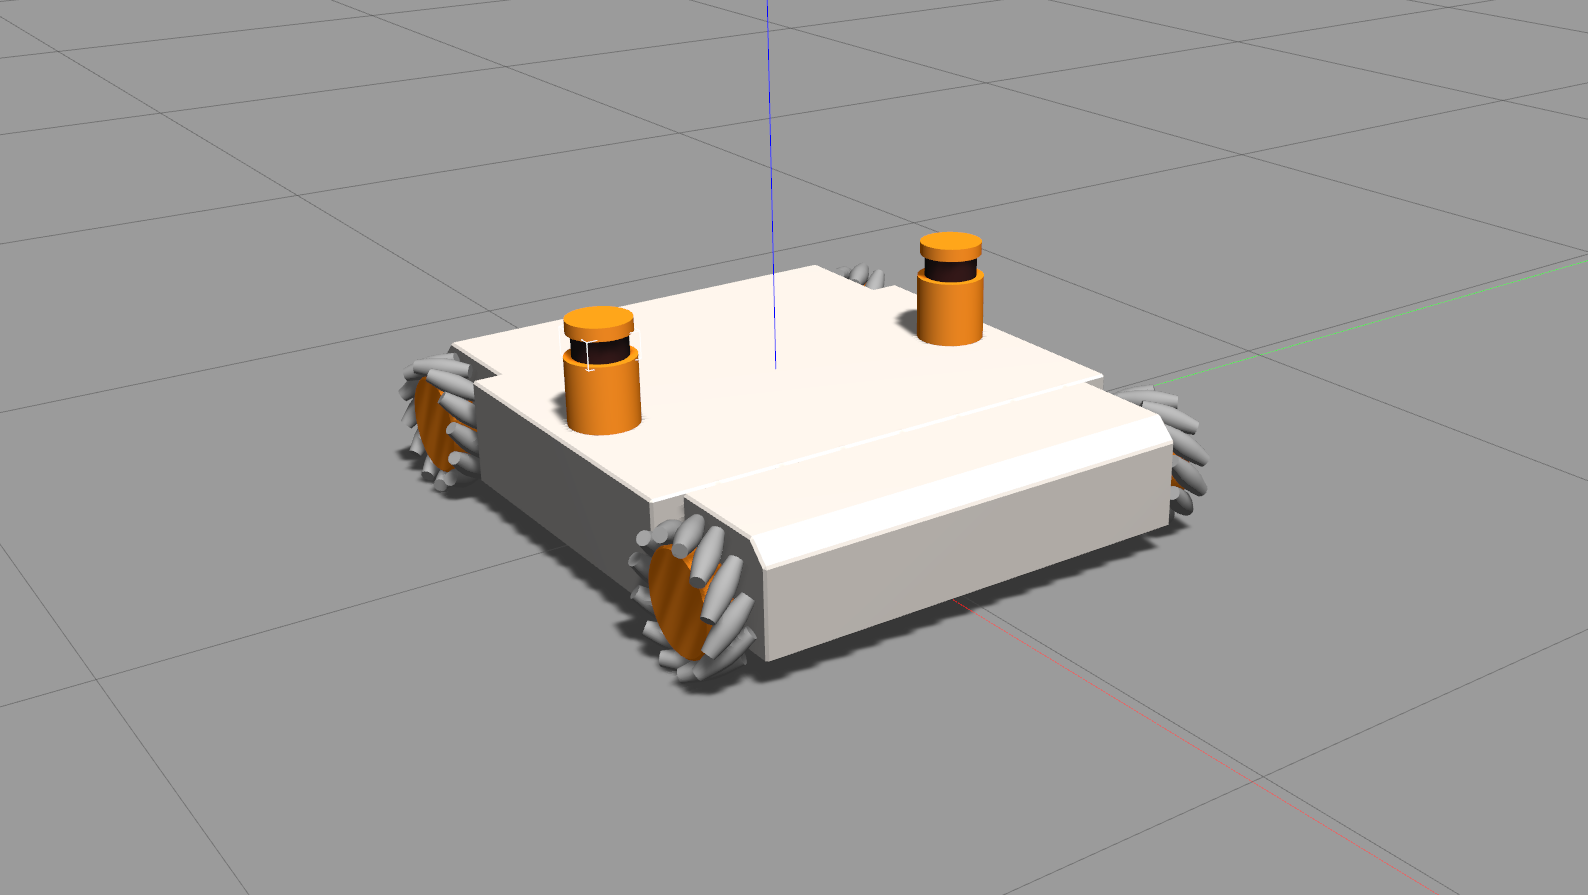
\includegraphics[scale=0.20]{./images/omnivelma_gz.png}
    \caption{Baza mobilna robota Velma w symulatorze Gazebo}
    \end{figure}
\end{frame}

\begin{frame}
    \frametitle{Baza mobilna Velmobil}
    Pojazd Velmobil posiada \cite{walas}:  
    \begin{itemize}
        \item 4 koła szwedzkie
        \item dwa skanery laserowe LIDAR
        \item jednostkę inercyjną
        \item enkodery % jakie enkodery
    \end{itemize}
\end{frame}